\chapter{Обзор подходов к компиляции гетерогенных приложений}\label{ch:overview}

\section{Логическая модель API для GPGPU}\label{sec:overview/api}

При работе с графическими API для вычислений (такими как OpenCL, SYCL, Cuda и прочие), программисту приходится иметь дело с несколькими уровнями памяти.
Базовое разделение это \textbf{память хоста} -- память хостовой машины, обычно это что-то вроде обычной RAM и \textbf{память устройства}, устроенная гораздо сложнее.

В простом случае память устройства бывает следующих видов:

\begin{itemize}
\item \textbf{Глобальная} -- память на устройстве обычно большого объёма и доступная каждому EU.
\item \textbf{Виртуальная разделяемая} -- участки памяти непосредственно отображаемые на память хоста.
\item \textbf{Константная} -- память, изменение которой в программах выполняемых на устройстве запрещено.
\item \textbf{Локальная} -- память доступная только потокам внутри рабочей группы.
\item \textbf{Приватная} -- память (обычно очень небольшое её количество) доступная только конкретному EU.
\end{itemize}

Обычно тип памяти напрямую запрашивается при работе с API как на листинге~\cref{lst:oclapi}.

\begin{ListingEnv}[!h]
    \captiondelim{ } 
    \caption{Пример запроса глобального буффера в OpenCL API}\label{lst:oclapi}
    \begin{lstlisting}[language={[ISO]C++}]
  cl_context Context;
  cl_mem Buf;
  cl_int Err;
  Context = clCreateContextFromType(NULL, CL_DEVICE_TYPE_GPU, NULL, 
                                    NULL, &Err);
  // .....
  Buf = clCreateBuffer(Context, CL_MEM_READ_WRITE, BUFSZ * sizeof(int), 
                       NULL, &Err);
    \end{lstlisting}
\end{ListingEnv}

В некоторых случаях компилятор может оптимизировать работу с памятью, например сделав stateless to stateful преобразование и тогда этот буфер окажется в satteful памяти (при соблюдении ряда условий).

Но логическая модель это не о том, что на самом деле, это о том, что видит программист.

\begin{figure}[ht]
    \centerfloat{
        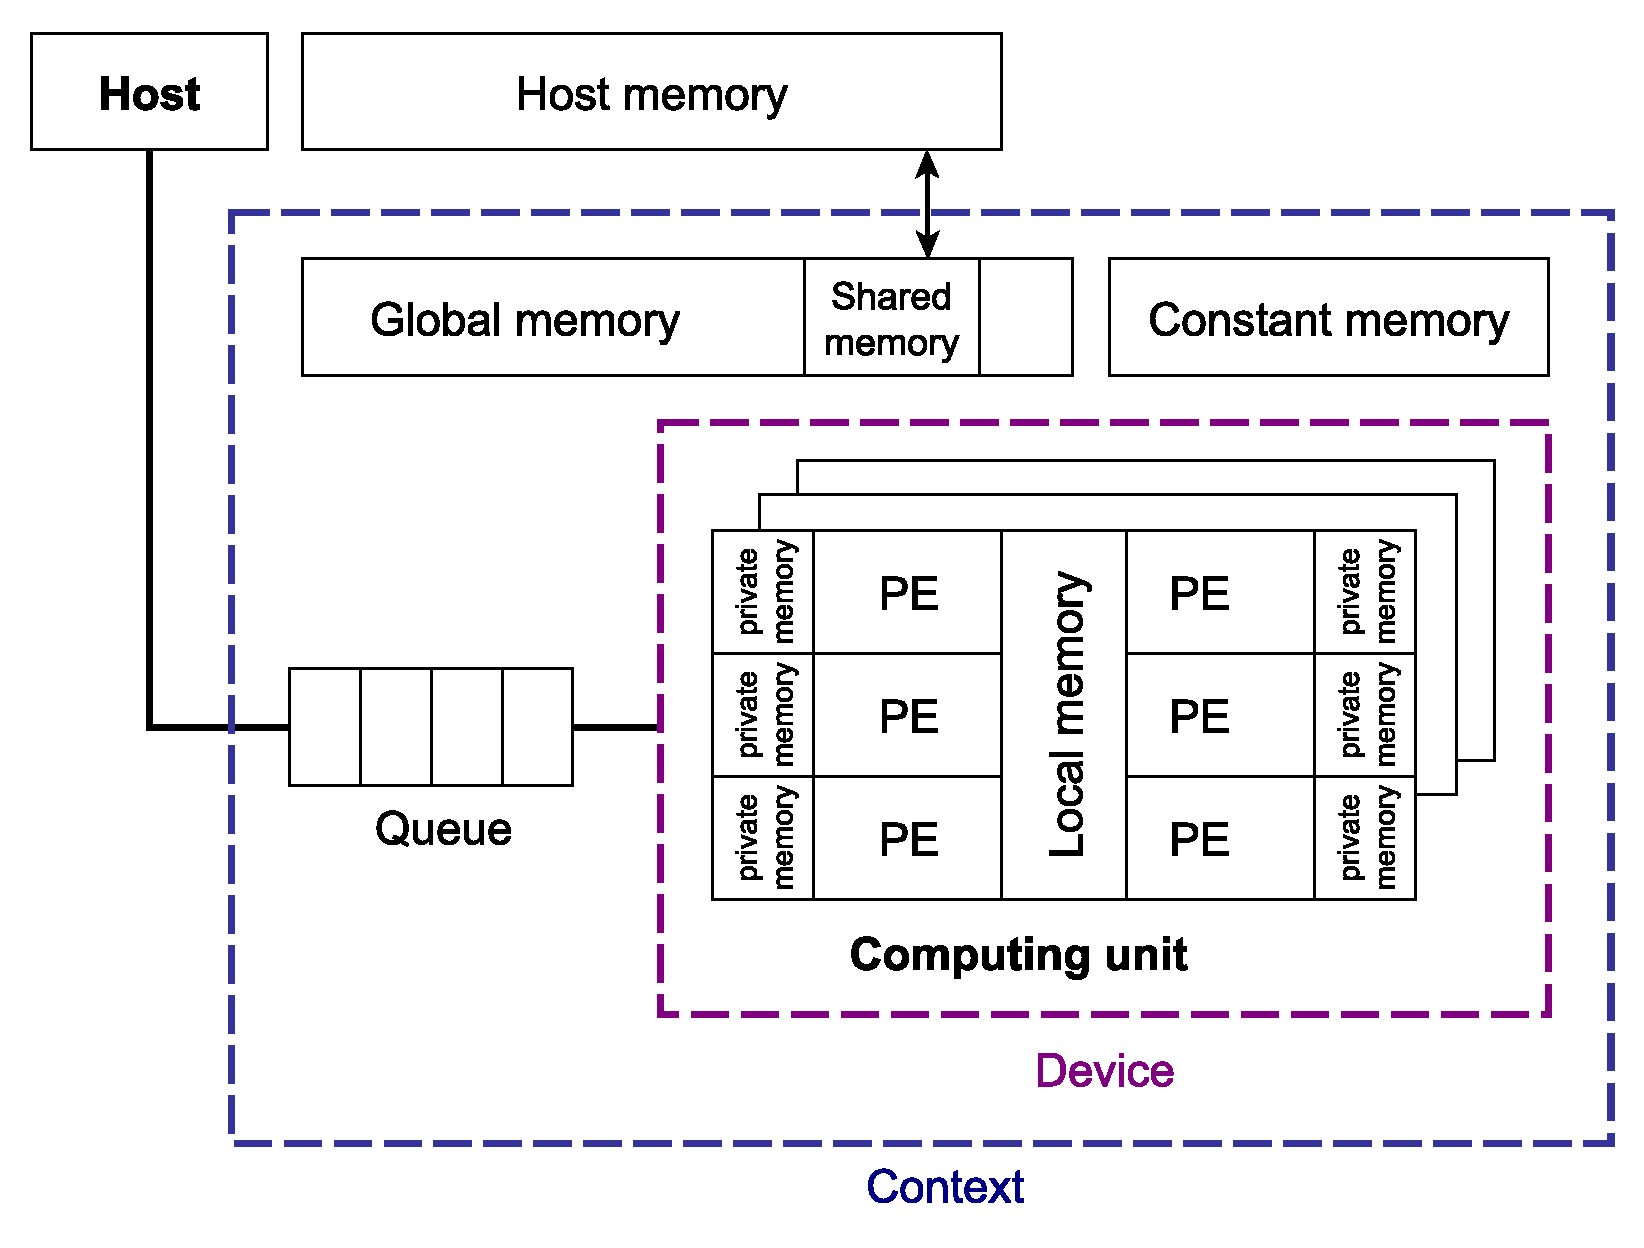
\includegraphics[scale=0.6]{Vladimirov/images/logical-memory.pdf}
    }
    \caption{Логическая модель памяти}\label{fig:logical-memory}
\end{figure}

Логическая модель памяти, характерная для таких API, как OpenCL и SYCL, представлена на рисунке~\cref{fig:logical-memory}

\section{Векторный характер графических систем команд}\label{sec:overview/hw}

Все гетерогенные вычисления нужны в основном затем, чтобы максимизировать производительность.
Для этих целей в средней видеокарточке используемой в гетерогенных системах обычно просто нет операционной системы -- её драйвер это драйвер операционной системы хоста.
В связи с эти для таких устройств (это верно и для GPU и для NPU) характерно.

\begin{enumerate}
\item Отсутствие накладных расходов на переключение контекста (нет OS).
\item Сравнительно далёкая и дорогая глобальная память.
\item Часто отсутствие кешей и короткий конвейер.
\end{enumerate}

Всё это мотивирует большие регистровые файлы.

\begin{figure}[ht]
    \centerfloat{
        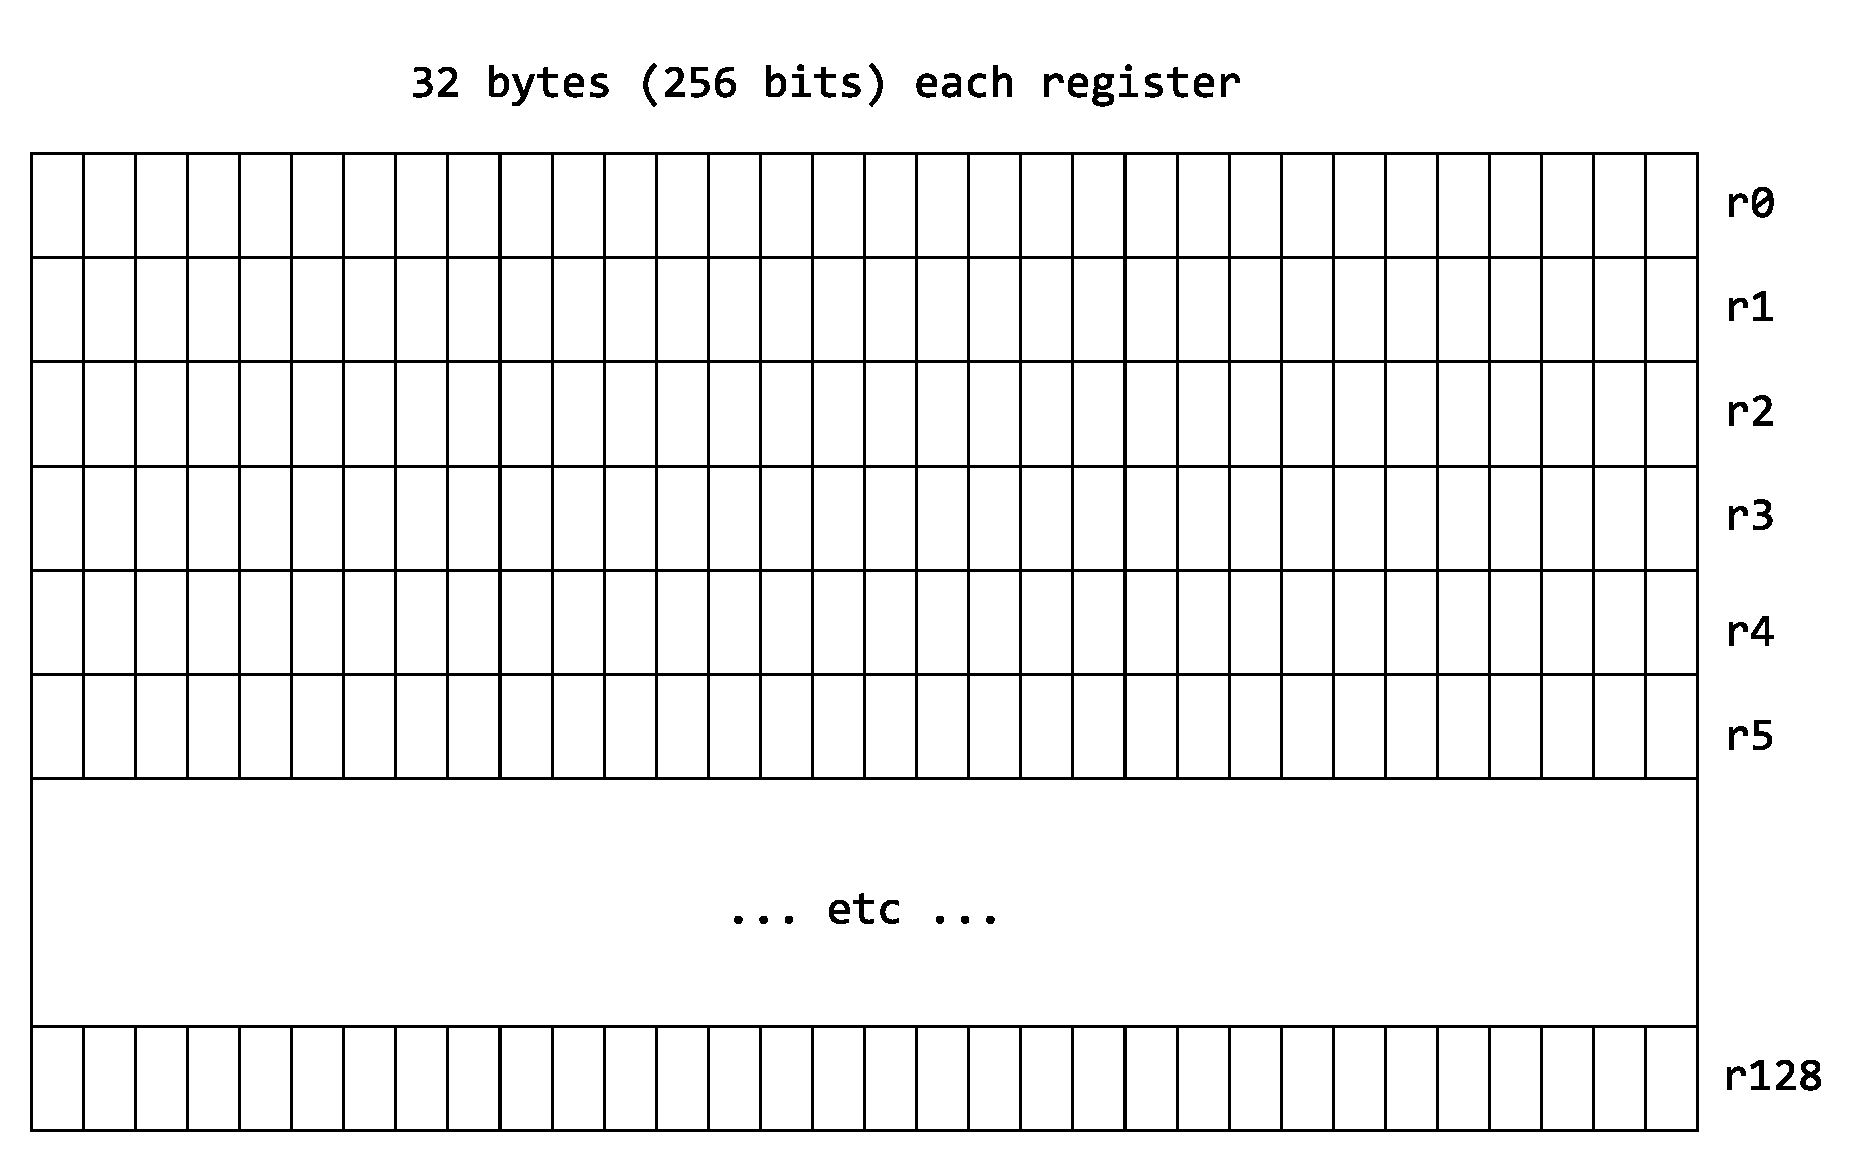
\includegraphics[scale=0.6]{Vladimirov/images/genisa-addressing-base.pdf}
    }
    \caption{Схема регистрового файла}\label{fig:genisa-addressing-base}
\end{figure}

Схема регистрового файла представлена на рисунке~\cref{fig:genisa-addressing-base}

Вовсе не всегда работа с большими регистровыми файлами удобна.

\section{Подходы к векторизации}\label{sec:overview/vectorizing}

Скалярная ISA и скалярное API (Cuda, NVPTX). Гибкая векторизация за счёт механизмов HW.
Сложное и дорогое железо.

Векторная ISA и скалярное API (OpenCL, SYCL). Векторизация после основных оптимизаций как часть кодогенерации.
Проблемы с векторизацией внешних циклов.
Необходимость SIMDX-dispatch, влияние на распределение регистров.

Векторная ISA и векторное API (CM) с ручным управлением регистровым файлом.
Минимальная роль компилятора.
Крайне сложное программирование.


\FloatBarrier
